\subsection{问题四的模型建立与求解}

问题四继续使用问题三的行动时间计算、示向区域递推、最小包围圆、可靠清除点、清除邻域偏移和终止判断，本节不再重复这些结论的证明，只讨论定向干扰源带来的新增状态与决策方法。

\subsubsection{定向可见性与联合状态}

设频道 $j$ 的干扰源位置为 $x_j\in\mathcal D$，有效接收半径为 $R_j\in[1000,1500]$，类型为 $\kappa_j$。当 $\kappa_j$ 为定向时，再以 $\psi_j$ 表示最大场强方向，并记
\begin{equation}
  u(\psi_j)=
  \left(
    \cos\frac{\pi\psi_j}{180},
    \sin\frac{\pi\psi_j}{180}
  \right)^{\mathsf T}.
  \label{eq:q4-direction-vector}
\end{equation}

对联合状态 $\xi=(x,R,\psi,\kappa)$，定义检测点 $s$ 的可接收指示量

\begin{equation}
  V(\xi,s)=
  \mathbf 1_{\{\|s-x\|_2\leq R\}}
  \begin{cases}
    1, & \kappa=\text{全向},\\
    \mathbf 1_{\{u(\psi)^{\mathsf T}(s-x)\geq0\}},
       & \kappa=\text{定向}.
  \end{cases}
  \label{eq:q4-visibility}
\end{equation}

定向接收须同时满足距离与发射正面限制；无信号不能直接用于删除位置圆盘。

对每个已发现频道，除问题三已有的位置外近似 $\widehat K_j$ 外，再维护有限可能状态集合
\begin{equation}
  \Xi_j=
  \left\{\xi_\ell=(x_\ell,R_\ell,\psi_\ell,
  \kappa_\ell,w_\ell)\right\}_{\ell=1}^{L_j},
  \qquad \sum_{\ell=1}^{L_j}w_\ell=1.
  \label{eq:q4-state-set}
\end{equation}

其中位置取不超过 $12$ 个代表点，半径取 $1000$、$1250$、$1500\ \mathrm m$，定向角按
$10^\circ$ 等间隔并补充历史检测方向及其 $\pm90^\circ$ 边界。全向类和定向类初始权重各取 $0.5$，
更新后重新归一化。

可能状态须与全部历史结果相容：无信号要求 $V=0$，近距离要求 $V=1$ 且距离不超过
$5\ \mathrm m$，有效示向度还要求真实方位落在误差范围内。因此
\begin{equation}
  \Xi_j^{(m)}=
  \left\{\xi\in\Xi_j^{(m-1)}:
  \xi\text{ 与 }(s_m,y_m)\text{ 相容}\right\}.
  \label{eq:q4-state-update}
\end{equation}

有限状态利用无信号信息选点，连续位置区域仍仅按有效示向度更新，以保持凸性和保守包含。

\subsubsection{二十五个三角网驻留点的初始扫描}

问题三的八点布局只保证任意源位置附近存在一个驻留点。若该点位于定向源背面，即使距离小于 $1000\ \mathrm{m}$ 也可能收不到信号。为同时控制距离和接近方向，本文在平面上建立等边三角网。

取三角网边长 $d_4=985\ \mathrm{m}$，平移参数 $\gamma_1=\gamma_2=0.112$，令
\begin{equation}
  Q_{ij}=d_4
  \left(
    i+\gamma_1+\frac{j+\gamma_2}{2},
    \frac{\sqrt3}{2}(j+\gamma_2)
  \right),
  \qquad i,j\in\mathbb Z.
  \label{eq:q4-triangular-lattice}
\end{equation}

保留所有与 $\mathcal D$ 相交的网格三角形，其顶点并集为 $\mathcal P_4$；上述参数得到
$25$ 个驻留点和 $33$ 个三角形。

机器狗从原点按最近邻构造开放顺序，再以确定性 $2$-opt 改进；该顺序不作为最短路径结论。
驻留点、访问顺序及接收半圆见图~\ref{fig:q4-triangular-scan}。

\begin{figure}[H]
  \centering
  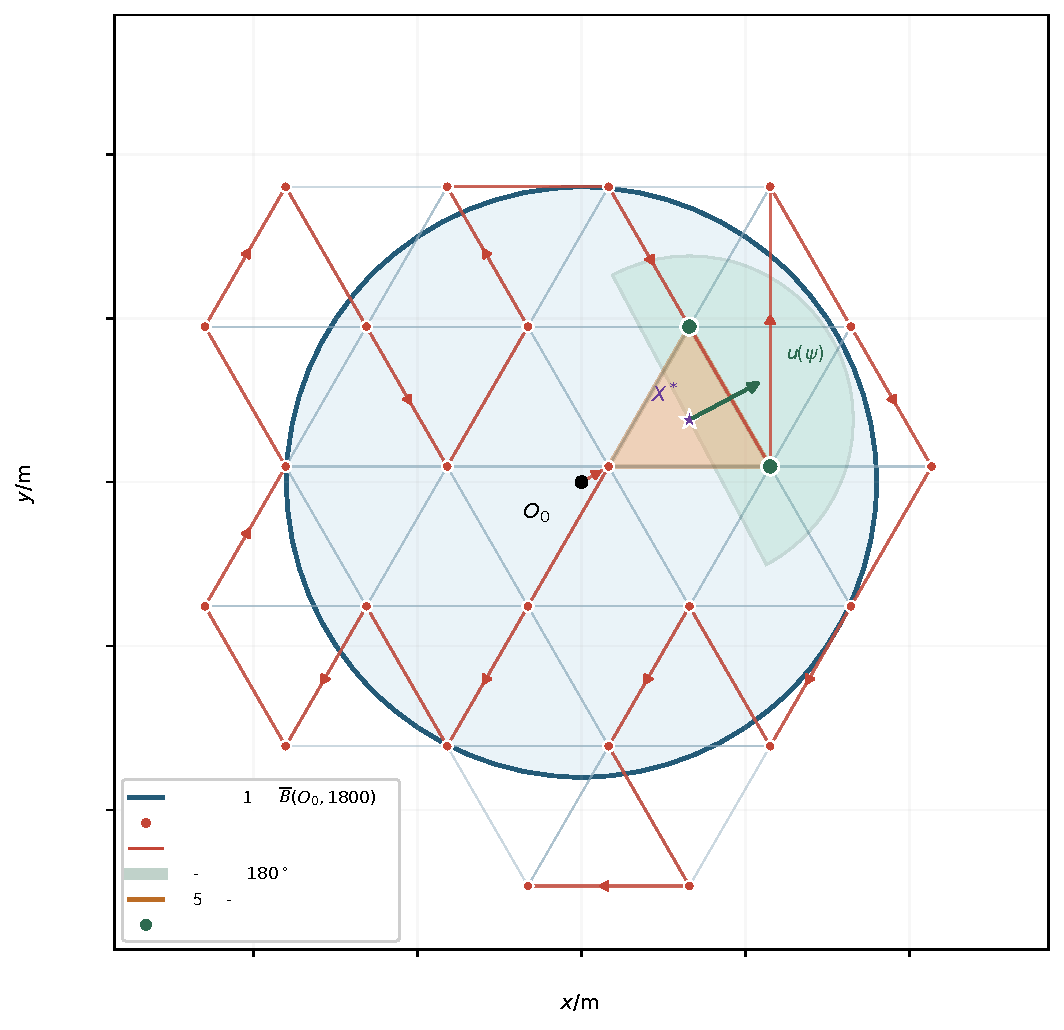
\includegraphics[width=0.83\textwidth]{figures/q4-triangular-scan.pdf}
  \caption{三角网扫描及定向覆盖：红线表示访问顺序，源 $X^*$ 的绿色接收半圆至少包含所在三角形的一个顶点}
  \label{fig:q4-triangular-scan}
\end{figure}

\noindent\textbf{命题 5：}{\kaishu 当三角网边长 $d_4\leq R_{\min}$ 时，集合 $\mathcal P_4$ 能够保证目标圆形区域内任一全向或定向干扰源至少在一个驻留点被发现。}

\noindent\textbf{证明：}
任取 $x\in\mathcal D$，存在保留的网格三角形 $T=\operatorname{conv}\{A,B,C\}$ 包含 $x$。
等边三角形直径等于边长，故
\begin{equation}
  \|A-x\|_2,\ \|B-x\|_2,\ \|C-x\|_2
  \leq d_4\leq R_{\min}.
  \label{eq:q4-triangle-distance}
\end{equation}

全向源在三个顶点均可接收。对定向源，将 $x$ 写成三顶点的凸组合；若三点均严格位于背面，则
\begin{equation}
  \begin{aligned}
    0&=u(\psi)^{\mathsf T}
    \left(\lambda_AA+\lambda_BB+\lambda_CC-x\right)\\
    &=\sum_{Q\in\{A,B,C\}}\lambda_Q u(\psi)^{\mathsf T}(Q-x)<0,
  \end{aligned}
\end{equation}

矛盾，故至少一个顶点同时满足方向与距离条件。\hfill$\square$

每个驻留点检测尚未清除的频道：近距离时原地清除，有效示向度时更新 $\widehat K_j$ 和
$\Xi_j$，无信号时仅更新 $\Xi_j$。扫描结束后，未发现频道归入无源集合。

\subsubsection{四侧探测组与局部三角网}

扫描后选择区域中心距当前位置最近的未处理频道；满足可靠条件则清除，否则构造多方向探测组。

设当前区域满足 $\widehat K_j\subseteq\overline B(c_j,r_j)$。

在中心的四个坐标轴方向设置
\begin{equation}
  \mathcal G_j^{\square}=
  \left\{
  c_j+(\rho_j,0),\ c_j+(0,\rho_j),
  c_j-(\rho_j,0),\ c_j-(0,\rho_j)
  \right\}.
  \label{eq:q4-four-sided-points}
\end{equation}

偏移量需要满足
\begin{equation}
  \sqrt2r_j<\rho_j\leq R_{\min}-r_j.
  \label{eq:q4-four-sided-condition}
\end{equation}

该区间非空要求 $r_j<R_{\min}/(1+\sqrt2)\approx414.214\ \mathrm m$；程序优先取接近 $200\ \mathrm m$ 的可行偏移量。

\noindent\textbf{命题 6：}{\kaishu 若式~\eqref{eq:q4-four-sided-condition} 成立，则对 $\widehat K_j$ 中任一可能源位置和任一发射方向，四侧探测点中至少有一个能够接收到该源信号。}

\noindent\textbf{证明：}
任取 $x\in\widehat K_j$。对任一四侧探测点 $q$，由三角不等式，
\begin{equation}
  \|q-x\|_2
  \leq\|q-c_j\|_2+\|c_j-x\|_2
  \leq\rho_j+r_j\leq R_{\min}.
  \label{eq:q4-four-distance}
\end{equation}

又由 $\|x-c_j\|_1\leq\sqrt2r_j<\rho_j$，源位于四点凸包内部；凸组合论证表明任一发射
正面至少包含一个满足距离条件的探测点。\hfill$\square$

四侧偏移不可行时，在外接矩形上铺设边长 $900\ \mathrm m$ 的局部三角网；探测组采用三种平移，
其方向覆盖理由与命题5相同。

探测组在得到有效示向度或近距离结果后结束；无信号时更新状态并选择组内剩余点。
每频道最多开始两个完整探测组。

\subsubsection{基于尾部风险的滚动选点}

利用有限联合状态，比较探测组的访问顺序及立即清除的预计时间，决定是否继续检测。

在区域外接矩形上建立边长 $27\ \mathrm m$ 的方格，其半对角线
$19.092\ \mathrm m<20\ \mathrm m$；按最近邻访问所得时间记为 $C_{\mathrm{base}}$，
再加入转向其他源的移动时间得到 $C_{\mathrm{clr}}$。实际清除仍沿用问题三的点列。

对访问顺序 $\pi$ 和状态 $\xi$ 累加行动时间；有效示向度分三种误差值预测新区域，并以
\begin{equation}
  \widehat C_{\mathrm{clr}}'
  =\max\left\{5,
  C_{\mathrm{base}}
  \left(\frac{r_j'}{r_j}\right)^2\right\}
  \label{eq:q4-clear-cost-scale}
\end{equation}

估计区域缩小后的清除时间，从而得到 $C(\pi,\xi)$。

将有限可能状态的相对权重归一化后，采用 Rockafellar 和 Uryasev 给出的等价优化形式~\cite{rockafellar2000}，以分位水平 $\alpha_R=0.9$ 的条件尾部均值评价较慢部分的完成时间：
\begin{equation}
  \mathcal R_{0.9}(\pi)
  =\min_{\eta\in\mathbb R}
  \left[
    \eta+\frac{1}{1-0.9}
    \sum_{\xi\in\Xi_j}w_\xi
    \bigl(C(\pi,\xi)-\eta\bigr)_+
  \right].
  \label{eq:q4-cvar}
\end{equation}

该指标关注耗时最长的 $10\%$ 状态。在线保留不超过 $8$ 个候选首点和 $48$ 个代表状态，记
\begin{equation}
  \pi^*=\operatorname*{arg\,min}_{\pi}\mathcal R_{0.9}(\pi).
\end{equation}

仅当
\begin{equation}
  \mathcal R_{0.9}(\pi^*)+\Delta_s<C_{\mathrm{clr}},
  \qquad \Delta_s=10\ \mathrm{s},
  \label{eq:q4-measure-or-clear}
\end{equation}

才执行 $\pi^*$ 的第一个测点，否则立即清除；每次响应后重新更新并求解，形成滚动决策。

计算上限为 $3\ \mathrm s$；状态为空、异常或超时则采用几何清除方案。有限状态只影响行动先后，
不改变清除覆盖保证。

\subsubsection{清除反馈、长尾处理与退出}

当定位半径 $r_j\leq19.9\ \mathrm{m}$ 时，直接沿用问题三的可靠清除点；当 $19.9<r_j\leq40\ \mathrm{m}$ 且尚未在中心试清除时，先在 $c_j$ 尝试一次。其余情况按式~\eqref{eq:q4-measure-or-clear} 在多方向探测与清除覆盖之间选择。

若在点 $y$ 清除失败，则由题设清除规则可知真实源位置满足 $\|x_j-y\|_2>20$。因此将有限可能状态更新为
\begin{equation}
  \Xi_j\leftarrow
  \left\{\xi\in\Xi_j:\|x_\xi-y\|_2>20\right\}.
  \label{eq:q4-failed-clear-update}
\end{equation}

清除失败后筛除有限状态并删除队首。满足剩余点数、位置和预计节省条件时可原地补测，每源至多三次；
连续失败 $8$ 次可再启动一次探测组，但不能替代完整覆盖。

多个未处理源按最近中心或清除点优先；清除成功后移入已清除集合，扫描未发现的频道移入无源集合。
满足式~\eqref{eq:q3-exit-condition} 时退出，完整过程见图~\ref{fig:q4-decision-tree}。

\begin{figure}[H]
  \centering
  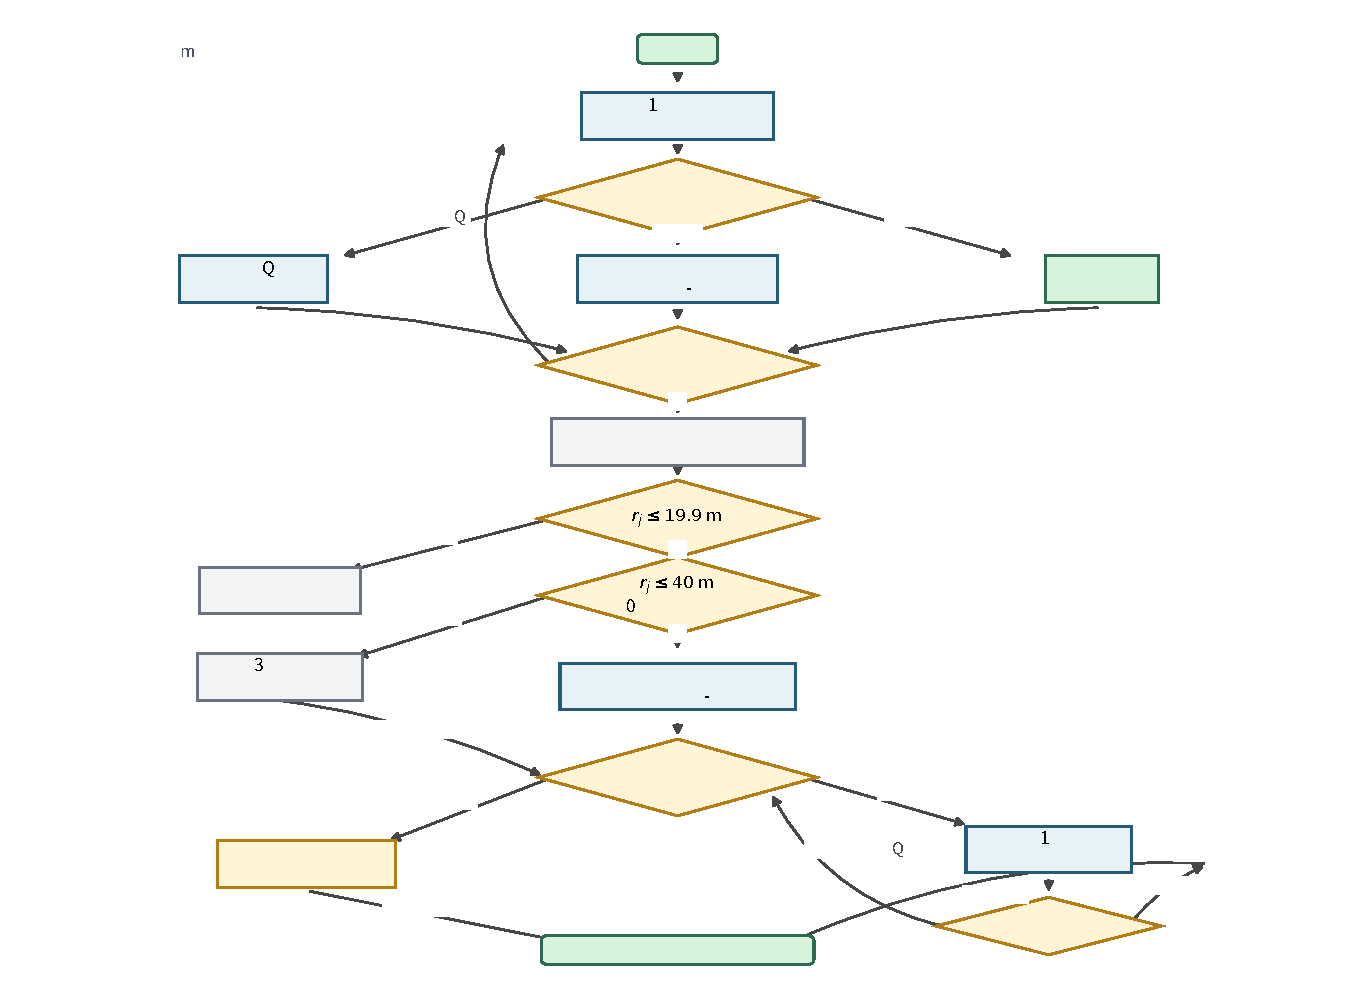
\includegraphics[width=0.98\textwidth]{figures/q4-decision-tree.pdf}
  \caption{问题四机器狗的定向扫描、联合状态更新、滚动选点与反馈清除决策树}
  \label{fig:q4-decision-tree}
\end{figure}
